\documentclass[a4paper]{article}

\usepackage[english]{babel}
\usepackage[utf8x]{inputenc}
\usepackage[T1]{fontenc}

\usepackage[a4paper,top=3cm,bottom=2cm,left=3cm,right=3cm,marginparwidth=1.75cm]{geometry}

\usepackage{amsmath}
\usepackage{graphicx}
\usepackage[colorinlistoftodos]{todonotes}
\usepackage[colorlinks=true, allcolors=blue]{hyperref}

\title{Manipulating Bitmap (BMP) images}
\author{Amin Azimov and Kamal Aghayev}

\begin{document}

\begin{figure}[t]
\centering
\begin{minipage}{.3\textwidth}
  \centering
  
\includegraphics[height=.4\linewidth]{unistra.jpg}
\end{minipage}
\begin{minipage}{.3\textwidth}
  \centering
  
\includegraphics[height=.3\linewidth]{ufaz.jpg}
\end{minipage}
\begin{minipage}{.3\textwidth}
  \centering
  
\includegraphics[height=.2\linewidth]{asoiu.png}
\end{minipage}
\end{figure}

\maketitle

\section{Introduction}

The goal of the project was:
\begin{itemize}
\item To understand BMP format.
\item To learn how to work with bytes instead of known variable types like integers, shorts etc.
\item To learn how to work with files.
\item To learn how to work with big and little endian values.
\item To learn basics of digital image processing.
\item Finally, to write a C code that crops a strip from a given image and to write a bash code that uses the C code to crop a strip from all images in the directory.
\end{itemize}

\begin{figure}[h]
\centering
\begin{minipage}{.45\textwidth}
  \centering
  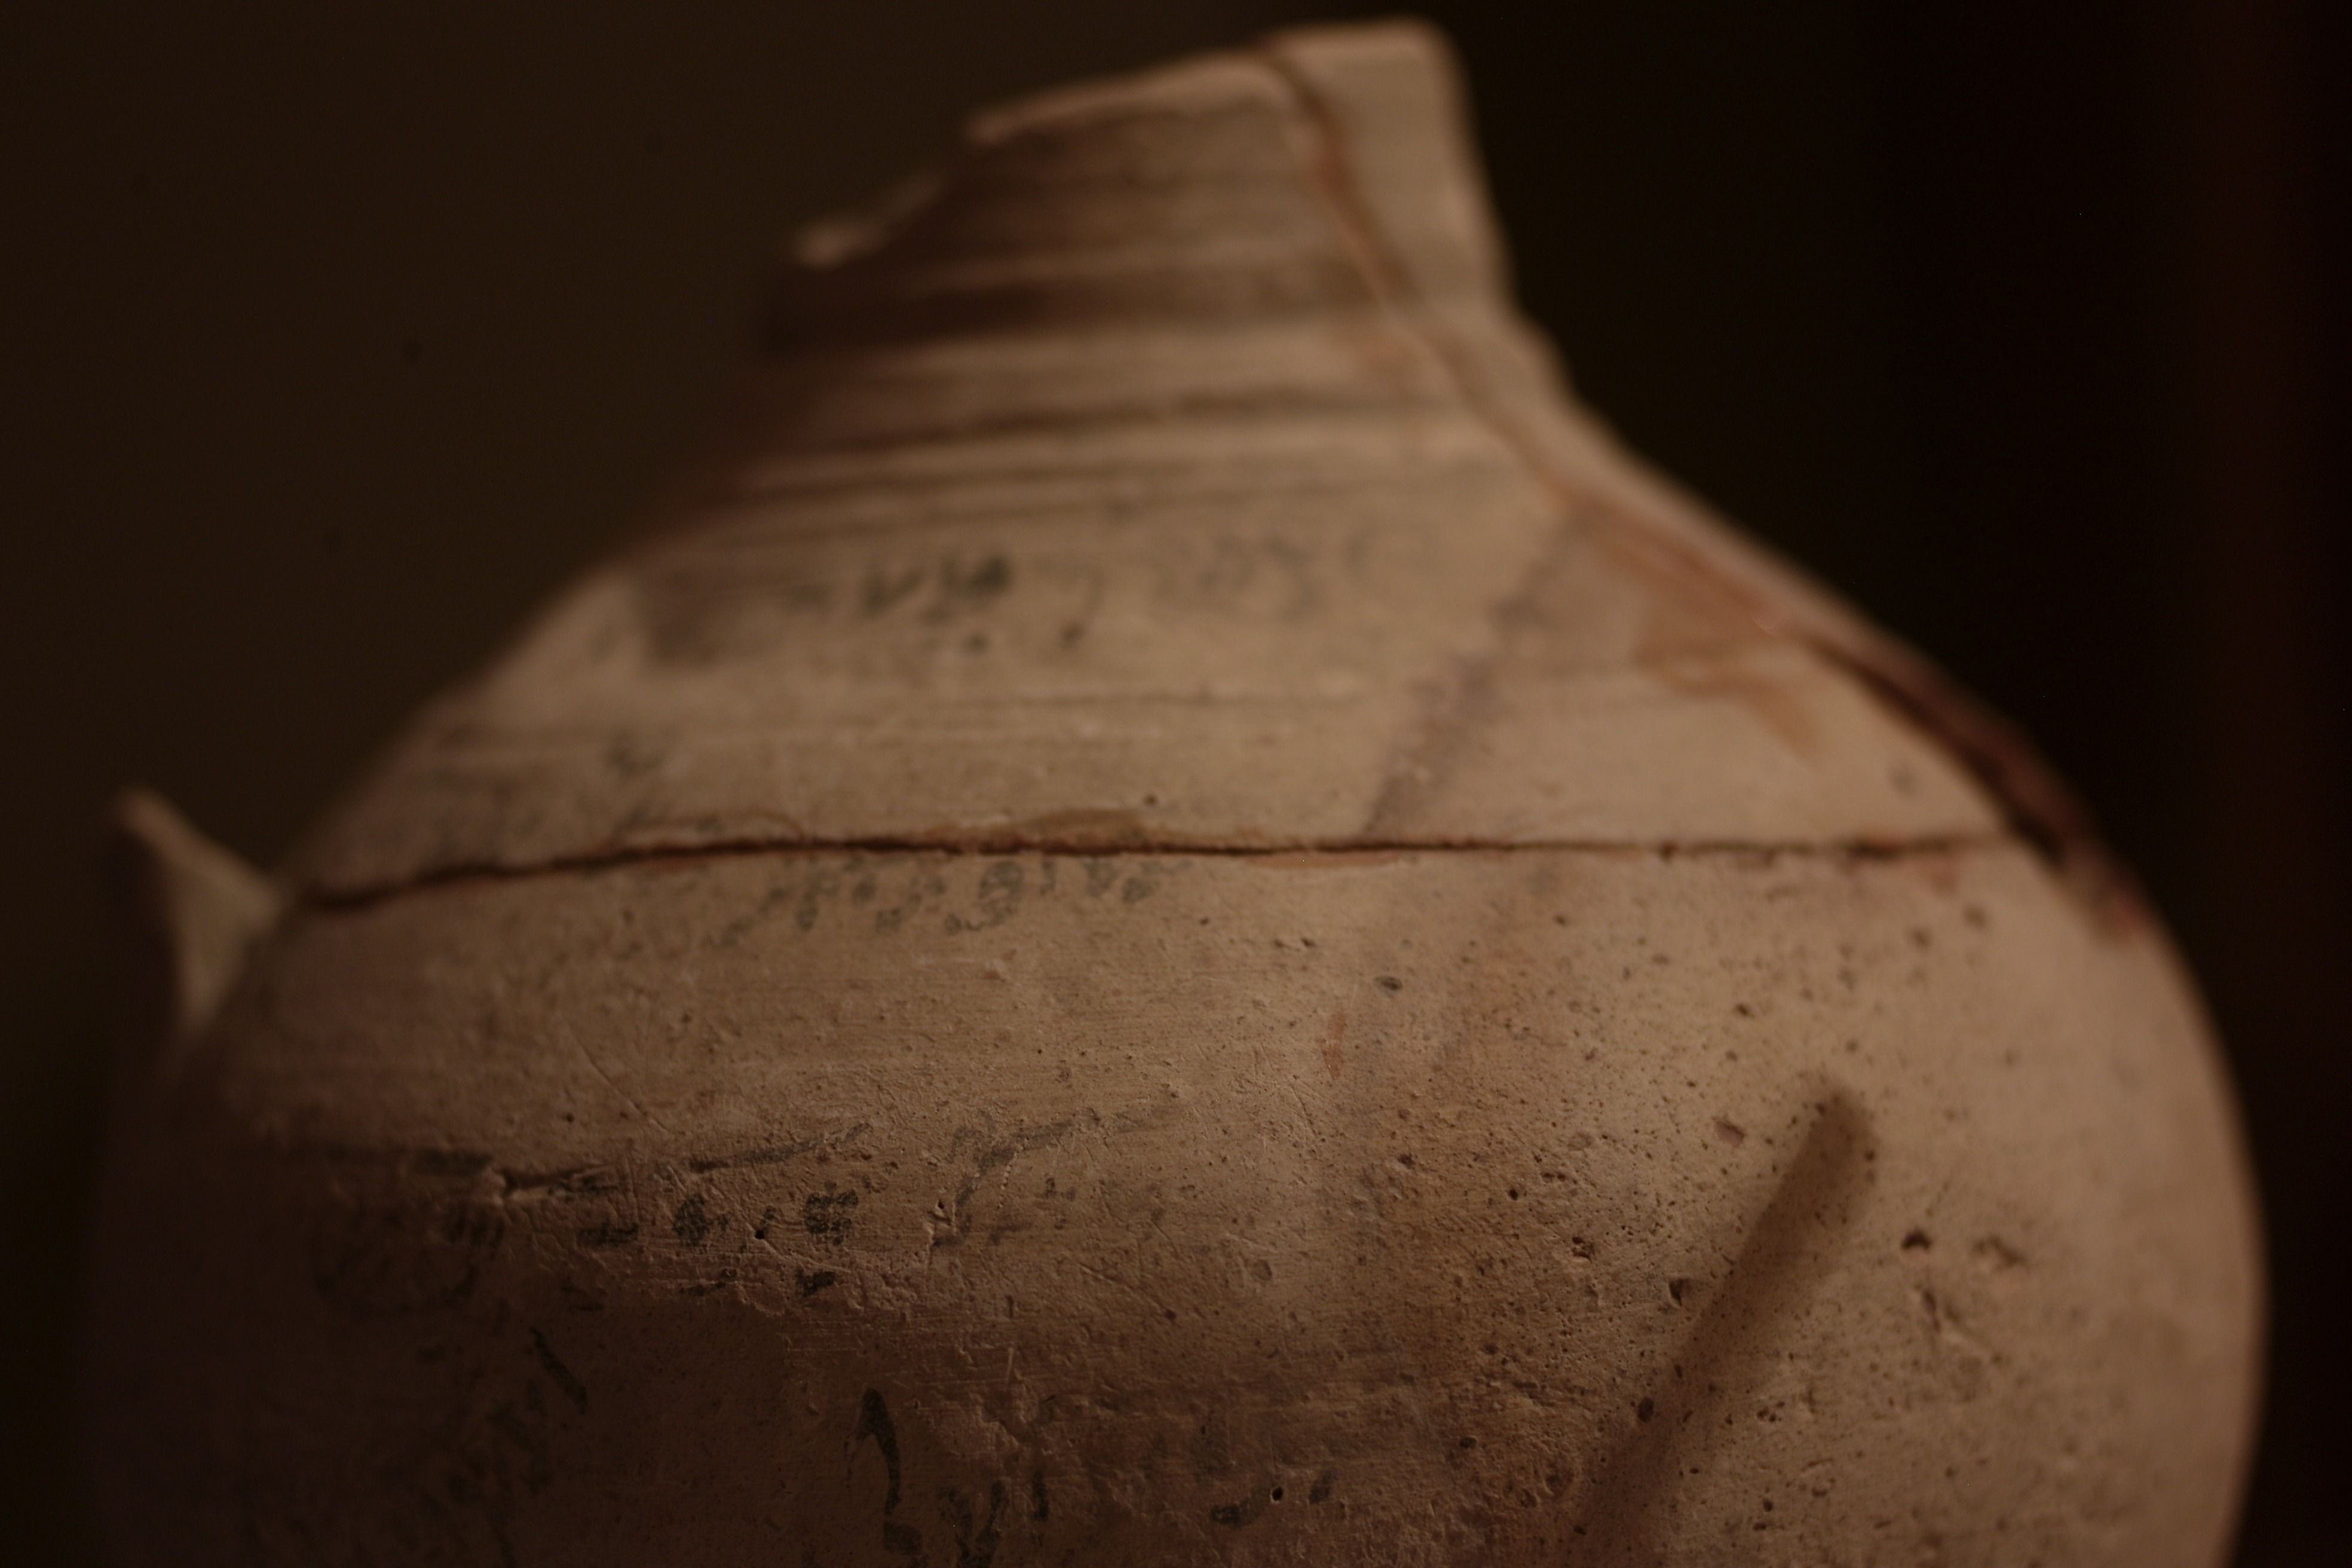
\includegraphics[height=.7\linewidth]{L1019472.jpg}
  \caption{\label{fig:pot1}Original image of pot.}
\end{minipage}
\begin{minipage}{.45\textwidth}
  \centering
  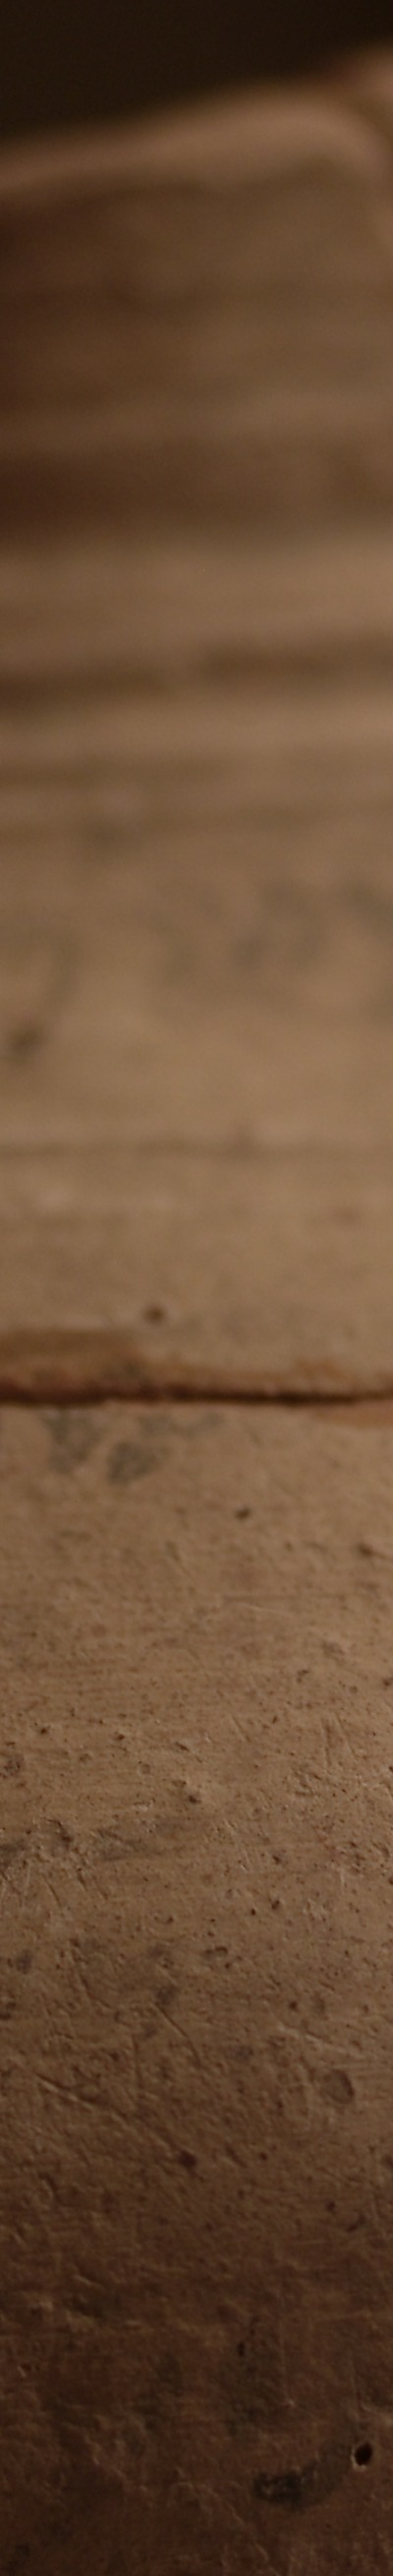
\includegraphics[height=.7\linewidth]{L1019472_S400.jpg}
  \caption{\label{fig:strip1}400 pixels strip of image of pot.}
\end{minipage}
\end{figure}

\section{Working Process}

\subsection{Algorithm}

Our work started from understanding the problem. We needed to crop the middle of the image. Cropping the middle of image in 2-dimensional(2D) array wouldn't be so difficult, but we have 1-dimensional(1D) array. Firstly, we need a formula to find a pixel at position ($x$, $y$) in 1D array. For this reason we used following formula:

\[pixels2D[y][x] = pixels1D[y * width + x],\]

where $x$ and $y$ are coordinates, and $width$ is a width of image\\\\
When we know how to access needed pixel in 1D array we can pass to the next problem. \\
BMP is composed of BMP header, DIB header and a bunch of pixels. After understanding what each byte is responding for we figured out that we need only following bytes to be stored separately:
\begin{itemize}
\item size of file
\item position of the first pixel in BMP file
\item width of image
\item height of image
\item number of bits per pixel
\end{itemize}
All values except $size Of File$ and $width Of Image$ from headers will be same in original and strip images. So to be more efficient we can read only these values from headers separately and store headers all bytes together in one array.\\
Finally we pass to pixels. First of all we read all pixels from an original file to an array of $size Of File - size of Headers$ elements. After copying all the pixels into a 1D array all we need is to copy needed pixels into a new BMP image.\\
After we have all needed data we can create a new BMP file and copy paste there headers. As it was said before we need to change values of $width Of Omage$ and $size Of Image$(i.e. 2-5 and 19-22 bytes). Width of image is a $size Of Strip$ that should be given by a user. To calculate $size Of Image$ we need to use following formula:

\[size Of Image = size Of Strip * height Of Image * bytes Per Pixel + size Of Headers,\]
where $bytes Per Pixel = bits Per Pixel / 8$.\\

To get a strip from image we copied all the pixels into 1D array. Now we need to write into a new BMP file only needed pixels(i.e. only middle $size Of Strip$ pixels). The solution when we stored pixels in 1D array was that we stored each byte separately. So for this reason to get ($x$, $y$) pixel we need to modify our previous formula as follows:
\[piexls2D[y][x] = pixel1D[(y * width + x) * bytesPerPixel],\]


\subsection{Problems}
During our work we faced with several problems. The main problem was with padding. 

\begin{figure}[h]
\centering
\begin{minipage}{.45\textwidth}
  \centering
  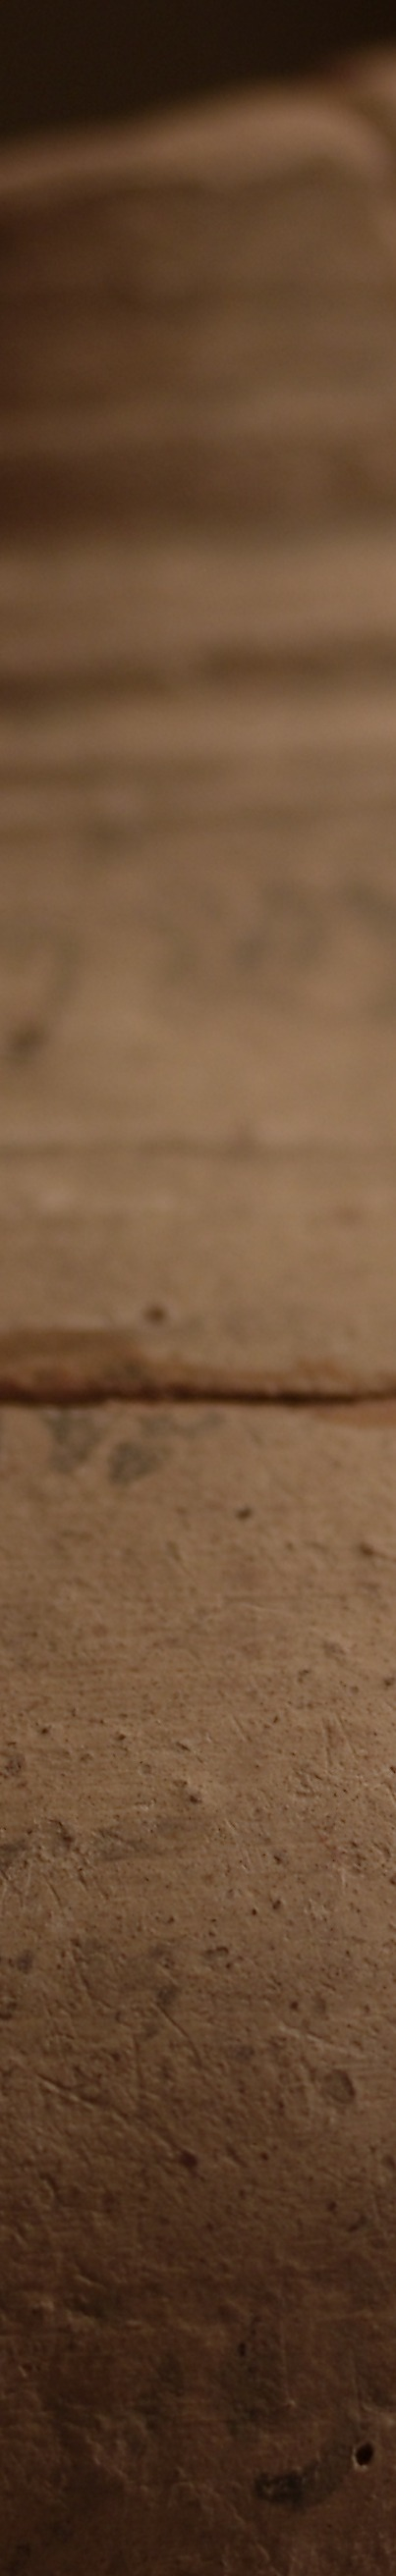
\includegraphics[height=.7\linewidth]{L1019472_S403_with_padding_.jpg}
  \caption{\label{fig:strip2}403 pixels strip image with padding.}
\end{minipage}
\begin{minipage}{.45\textwidth}
  \centering
  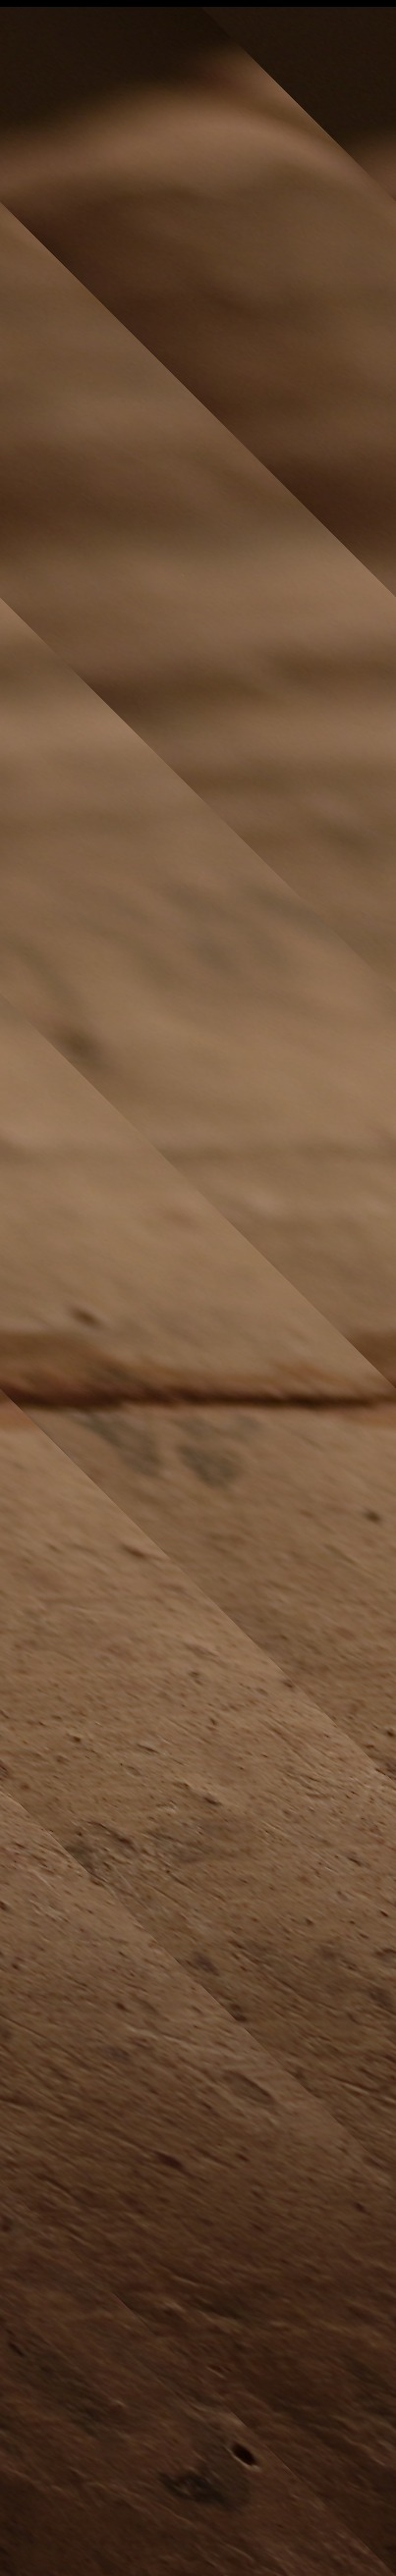
\includegraphics[height=.7\linewidth]{L1019472_S403_without_padding_.jpg}
  \caption{\label{fig:strip3}403 pixels strip image without padding.}
\end{minipage}
\end{figure}

After some research(we somehow skipped this in PDF description of project) we found information that the number of bits in a row in BMP file should be multiple of 32. So the solution was the following formula:
\[padding = (4 - (size Of Strip * bytes Per Pixel) \% 4) \% 4\]
After copying each row into a new BMP file we just added $padding$ zeros into a file.
\\
\\
The last piece of puzzle was to write a bash code that makes a strip of a given size(if size is not defined size of strip will be equal to 100 as default).

\section{Results}
As a result of our project we did:
\begin{itemize}
\item Learned how to deal with BMP format
\item Learned how to deal with bytes instead of dealing with known variable types 
\item Learned the very basics of image processing
\item Revised how to work with files
\item Revised how to write a bash code
\end{itemize}
Working on this file we can also say that we overdid our goals since we also learned the basics of \LaTeX \\\\
As a result we have a C code that crops a strip of given size from a given BMP file and saves it into new file. It also has a manual for users that don't realize how to use it. We have a bash code that uses the C code to crop strips of a given size from all the files in the directory. Like C code it also has a manual for users\\
In addition we have README file where you can find manual for whole project.\\\\
P.S. We wrote our code in a way that it can be easily modified to work with pixels for image processing. Now, to make some image processing we can easily use our code to read BMP file and then manage pixels in a way we want.

\end{document}